\documentclass[11pt]{article}\usepackage[]{graphicx}\usepackage[]{color}
%% maxwidth is the original width if it is less than linewidth
%% otherwise use linewidth (to make sure the graphics do not exceed the margin)
\makeatletter
\def\maxwidth{ %
  \ifdim\Gin@nat@width>\linewidth
    \linewidth
  \else
    \Gin@nat@width
  \fi
}
\makeatother

\definecolor{fgcolor}{rgb}{0.345, 0.345, 0.345}
\newcommand{\hlnum}[1]{\textcolor[rgb]{0.686,0.059,0.569}{#1}}%
\newcommand{\hlstr}[1]{\textcolor[rgb]{0.192,0.494,0.8}{#1}}%
\newcommand{\hlcom}[1]{\textcolor[rgb]{0.678,0.584,0.686}{\textit{#1}}}%
\newcommand{\hlopt}[1]{\textcolor[rgb]{0,0,0}{#1}}%
\newcommand{\hlstd}[1]{\textcolor[rgb]{0.345,0.345,0.345}{#1}}%
\newcommand{\hlkwa}[1]{\textcolor[rgb]{0.161,0.373,0.58}{\textbf{#1}}}%
\newcommand{\hlkwb}[1]{\textcolor[rgb]{0.69,0.353,0.396}{#1}}%
\newcommand{\hlkwc}[1]{\textcolor[rgb]{0.333,0.667,0.333}{#1}}%
\newcommand{\hlkwd}[1]{\textcolor[rgb]{0.737,0.353,0.396}{\textbf{#1}}}%

\usepackage{framed}
\makeatletter
\newenvironment{kframe}{%
 \def\at@end@of@kframe{}%
 \ifinner\ifhmode%
  \def\at@end@of@kframe{\end{minipage}}%
  \begin{minipage}{\columnwidth}%
 \fi\fi%
 \def\FrameCommand##1{\hskip\@totalleftmargin \hskip-\fboxsep
 \colorbox{shadecolor}{##1}\hskip-\fboxsep
     % There is no \\@totalrightmargin, so:
     \hskip-\linewidth \hskip-\@totalleftmargin \hskip\columnwidth}%
 \MakeFramed {\advance\hsize-\width
   \@totalleftmargin\z@ \linewidth\hsize
   \@setminipage}}%
 {\par\unskip\endMakeFramed%
 \at@end@of@kframe}
\makeatother

\definecolor{shadecolor}{rgb}{.97, .97, .97}
\definecolor{messagecolor}{rgb}{0, 0, 0}
\definecolor{warningcolor}{rgb}{1, 0, 1}
\definecolor{errorcolor}{rgb}{1, 0, 0}
\newenvironment{knitrout}{}{} % an empty environment to be redefined in TeX

\usepackage{alltt}
%\documentclass[11pt]{scrartcl}
\usepackage{amsmath, amsfonts, amssymb}
\usepackage{adjustbox}
\usepackage{fullpage}
\usepackage{epsfig}
\usepackage{hyperref}
\hypersetup{
     colorlinks   = true,
     citecolor    = black
}
\hypersetup{linkcolor=black}

\usepackage{multicol}

\renewcommand{\baselinestretch}{1.4}
\usepackage{float}
\usepackage{wrapfig}

\title{High Resolution Identification of Protein-DNA Binding Events
  and Quality Control for ChIP-exo data\vspace*{\fill}}

\author{Rene Welch\\Preliminary Examination\\Department of Statistics, University of Wisconsin-Madison}

\date{December 1st, 2015}



%% commmands
%\usepackage{Sweave}
\IfFileExists{upquote.sty}{\usepackage{upquote}}{}
\begin{document}

\newcommand{\sig}{\sigma^{70}}


\maketitle

\vspace*{\fill}

\textbf{Committee Members:}

\textbf{Professor S\"und\"uz Kele\c{s}}, Department of Statistics,
Department of Biostatistics and Medical Informatics

\textbf{Professor Karl Broman}, Department of Biostatistics and
Medical Informatics

\textbf{Professor Colin Dewey}, Department of Computer Sciences,
Department of Biostatistics and Medical Informatics

\textbf{Professor Christina Kendziorski}, Department of Biostatistics
and Medical Informatics

\textbf{Professor Ming Yuan}, Department of Statistics

\thispagestyle{empty}


\newpage

\tableofcontents

\newpage

\listoffigures

\newpage


\section*{Abstract}

    Recently, ChIP-exo has been developed to investigate protein-DNA
    interaction in higher resolution compared to popularly used
    ChIP-Seq. Although ChIP-exo has drawn much attention and is
    considered as powerful assay, currently no systematic studies
    have yet been conducted to determine optimal strategies for
    experimental design and analysis of ChIP-exo. In order to address
    these questions, we evaluated diverse aspects of ChIP-exo and
    found the following characteristics of ChIP-exo data. First, the
    background of ChIP-exo data is quite different from that of
    ChIP-Seq data. However, sequence biases inherently present in
    ChIP-Seq data still exist in ChIP-exo data. Second, in ChIP-exo
    data, reads are located around binding sites much more tightly and
    hence, it has potential for high resolution identification of
    protein-DNA interaction sites, and also the space to allocate the
    reads is greatly reduced. Third, although often assumed in the
    ChIP-exo data analysis methods, the ``peak pair'' assumption does
    not hold well in real ChIP-exo data. Fourth, spatial resolution of
    ChIP-exo is comparable to that of PET ChIP-Seq and both of them
    are significantly better than resolution of SET ChIP-Seq. Finally,
    for given fixed sequencing depth, ChIP-exo provides higher
    sensitivity, specificity and spatial resolution than PET
    ChIP-Seq.

    We provide a quality control pipeline which visually assess
    ChIP-exo biases, library complexity and enrichment; and calculates
    a signal-to-noise measure. Also, we updated dPeak (Chung et al.,
    2012 \cite{dpeak}), which makes a striking balance in sensitivity,
    specificity and spatial resolution for ChIP-exo data analysis.

\newpage

\section{Introduction}
\label{sec:intro}


ChIP-exo (Chromatin Immunopecipitation followed by exonuclease
digestion and next generation sequencing) Rhee and Pugh, 2011
(\cite{exo1}) is the state-of-the-art experiment developed to attain
single base-pair resolution of protein binding site identification and
it is considered as a powerful alternative to popularly used ChIP-Seq
(Chromatin Immunoprecipitation coupled with next generation sequencing
) assay.

While the number of produced ChIP-exo data keeps increasing,
characteristics of ChIP-exo data and optimal strategies for
experimental design and analysis of ChIP-exo data are not fully
investigated yet, including issues of sequence biases inherent to
ChIP-exo data, choice of optimal statistical methods, and
determination of optimal sequencing depth. However, currently the
number of available ChIP-exo data is still limited and their
sequencing depths are still insufficient for such investigation. To
address this limitation we gathered ChIP-exo data from diverse
organisms: CTCF factor in human \cite{exo1}; ER factor in human and
FoxA1 factor in mouse (Serandour et al., 2013 \cite{exoillumina}); and
generated $\sig$ factor in Escherichia coli (E. Coli) under
aerobic ($ + O_2$) condition, and treated by rifampicin by 0 and 20
minutes.

DNA libraries generated by the ChIP-exo protocol seem to be less
complex than the libraries generated by ChIP-Seq (Mahony et al., 2015
\cite{exo_review}). Hence, most of current QC guidelines (Landt et
al., 2012 \cite{encode_qc}) may not be applicable on ChIP-exo,
additionally to our knowledge there are not established quality
control pipelines for ChIP-exo. To address this challenge, we suggest
a collection of quality control visualizations to understand which
biases are present in ChIP-exo data. Previous ChIP-exo analysis used
ChIP-Seq samples to compare the resolution between experiments
(\cite{exo1}, \cite{exo2}, \cite{exoillumina}); Carroll et al., 2014
\cite{carroll.qc} studied the use of the Strand-Cross Correlation
(SCC) (Kharchenko et al., 2008 \cite{strandcc}) and showed that by
filtering blacklisted regions the estimation of the SCC is
improved. However, this method requires to know blacklisted regions in
advance which may not be available, additionally using SCC may not be
useful since the peaks that are attained at the read and fragment
length are confused in a typical ChIP-exo SCC curve.  In our pipeline
we propose two out-the-shelf analysis: an enrichment plot and the
local normalized SCC cofficient.

In order to archive the potential benefits of ChIP-exo on protein
binding site identification, it is critical to understand which are
the important characteristics of ChIP-exo data and to use algorithms
that could fully utilize information available in ChIP-exo data. Rhee
and Pugh, 2011 \cite{exo1} discussed that reads in the forward and
reverse strand might construct peak pairs around bound protein, of
which heights were implicitly assumed to be symmetric. Hence, they
used the ``peak pair method'' that predicts the midpoint of two modes
of peak pairs as potential binding site. Mace (Wang et al., 2014
\cite{mace}), CexoR (Madrigal, 2015 \cite{cexor}) and peakzilla
(Bardet et al., 2013 \cite{peakzilla}), recently developed ChIP-exo
data analysis methods, are also based on this peak pair
assumption. However, appropriateness of such assumption was not fully
evaluated in the literature yet.  Furthermore, it is still unknown
which factors could affect protein binding site identification using
ChIP-exo data. In order to address this problem, we investigated
various aspects of ChIP-exo data by contrasting them with their
respective ChIP-Seq experiments.

Currently, research on statistical methods for ChIP-exo data is still
in its very early stage. Although many methods have been proposed to
identify protein binding sites from ChIP-Seq data (reviewed by
Wilbanks and Facciotti, 2012 \cite{evaluation} and Pepke and Wold,
2009 \cite{computation}), such as MACS (Zhang et al., 2008
\cite{macs}), CisGenome (Hongkai et al., 2008 \cite{cisgenome}) and
MOSAiCS (Kuan et al., 2009 \cite{mosaics}), these approaches reveal
protein binding sites in lower resolution, i.e., at an interval of
hundreds to thousands of base pairs. Furthermore, they report only one
``mode'' or ``predicted binding location'' per peak. Hence, these
methods are not appropriate to evaluate the potential of ChIP-exo data
for high resolution identification of protein binding sites. More
recently, deconvolution algorithms such as Deconvolution (Lun et al.,
2009 \cite{csdeconv}), GEM (Guo et al., 2012 \cite{gem}, an improved
version of Guo et al., 2010 \cite{gps} ) and PICS (Zhang et al., 2010
\cite{pics}) have been proposed to identify binding sites in higher
resolution using ChIP-Seq data. However, most of them are still not
tailored for ChIP-exo and PET and SET ChIP-Seq data in a unified
framework and as a result, currently available methods are not
appropriate for fair comparison between ChIP-exo and ChIP-Seq. To
address these limitations, we developed an improved of dPeak (Chung et
al., 2013 \cite{dpeak}), a high resolution binding site identification
(deconvolution) algorithm that we previously developed for PET and SET
ChIP-Seq data, so that it can also handle ChIP-exo data. The dPeak
algorithm implements a probabilistic model that accurately describes
the ChIP-exo and ChIP-Seq data generation process.

In this work, we demonstrate that the ``peak pair'' assumption of
Rhee and Pugh \cite{exo1} does not hold well in real ChIP-exo
data. Furthermore, we found that when we analyze ChIP-exo data from
eukaryotic genomes, it is important to consider sequence biases
inherent to ChIP-exo data, such as mappability and GC content in order
to improve sensitivity and specificity of binding site
identification. We evaluated several method to identify binding events
and dPeak outperforms or performs competitively respecto to GEM and
MACE when analyzing ChIP-exo data. More importantly, when comparable
number of reads is used for both ChIP-exo and ChIP-Seq, dPeak coupled
with ChIP-exo data provides resolution comparable to PET ChIP-Seq and
both significantly improve the resolution of protein binding site
identification compared to SET-based analysis with any of the
available methods.

\section{ChIP-exo and ChIP-Seq review}
\label{sec:exo}

\begin{wrapfigure}{l}{.4\textwidth}
\centering
\includegraphics{../figs/diagrams/ChIPexo_diagram.png}
\caption{ChIP-exo diagram. The only difference with ChIP-Seq is the
  second step, where an exonuclease enzyme is added and it diggest the
  DNA fragments starting from the 5' end until it finds a crosslink
  protein (this figure is taken from Furey, 2012 \cite{chipbeyond}).}
\label{fig:exo}
\end{wrapfigure}

ChIP-exo is based in a modification to the ChIP-seq protocol, where an
exonuclease enzyme is added and it diggests the fragments starting by
the 5' ends and stops until it finds a protein that is crosslinked to
the DNA.

ChIP-exo experiments first capture millions of DNA fragments
(150 - 250 bp in length) that the protein under study interacts with
using random fragmentation of DNA and a protein-specific
antibody. Then, exonuclease is introduced to trim 5' end of each DNA
fragment to a fixed distance from the bound protein. As a result,
boundaries around the protein of interest constructed with 5' ends of
fragments are located much closed to bound protein compared to
ChIP-Seq. This step is unique to ChIP-exo and could potentially
provide significantly higher spatial resolution compared to
ChIP-Seq. Finally, high throughput sequencing of a small region (25 to
100 bp) at 5' end of each fragment generates millions of reads or
tags.

Since this protocol is a modification to ChIP-Seq, some of its
characteristics are still maintained in ChIP-exo while several new are
being found. Rhee and Pugh, 2011 \cite{exo1}, showed that ChIP-exo
generated fragments are located around the binding events more tightly
than ChIP-Seq generated fragments. Hence, it is of utmost importance
to understand how this new protocol works, specifically we focused on
understanding which biases are mantained from ChIP-Seq to ChIP-exo,
which biases are specific to ChIP-exo, how the current ChIP-Seq QC
guidelines behave in ChIP-exo and we developed a new QC pipeline
specific to ChIP-exo. A typical example is shown in figure
\ref{fig:exo_example}, which shows the $\sig$ and $\beta'_f$ factors
(and the $\beta$ factor only on top) on a E. Coli genome's region:
First, both regions show that the $\sig$ sample is enriched; second
the $\sig$ sample in the ChIP-exo panel shows that its respective form
in the ChIP-Seq panel may be form of more binding events; and third,
either of the $\beta$ factors show that the complexity of the ChIP-exo
libraries may be lower in some cases, i.e. the peak is mapped with
fewer positions.

\begin{figure}[h!]
  \centering
  \includegraphics[width = .8 \textwidth,page = 107]{/p/keles/ChIPexo/volume5/OpenClosedComplexes/figs/peaks/ChIPseq_ChIPexo_peaks_rif20.pdf}
  \caption{An example of a PET ChIP-Seq peak compared to
    ChIP-exo. $\sig$, $\beta$ and $\beta_f'$ are subunits of
    the transcription initiation complex in E. Coli. Gene regions on
    the reverse strand are highlighted in light blue and the region
    was centered respect to ChIP-Seq $\sig$ summit. The library
    complexity is lower in ChIP-exo than in ChIP-Seq but the
    resolution is increased, this can be observed at the $\sig$
    peak that for ChIP-exo was created as the combination of at least
    three ChIP-exo ``sub-peaks''.}
  \label{fig:exo_example}
\end{figure}

\subsection{Current Quality Control Measures for ChIP-Seq}
\label{sec:QC_chipseq}

To our knowledge it doesn't exists a QC pipeline for ChIP-exo. Hence,
we analyzed how the current ChIP-Seq QC measures behave on ChIP-exo
data.

\begin{table}[h]
  \centering
  \caption{Usual quality control indicators applied to the $\sigma^{70}$ samples. PBC stands PCR-bottleneck coefficient, SSD for standardized standard deviation, NSC for normalized strand cross-correlation coefficient (Another measure related to the strand cross-correlation curve is the RSC was ommited since input sample usually don't exists for ChIP-exo). $\sig$ samples were given by Robert Landick, FoxA1 and ER samples are from Serandour et al., 2013 \cite{exoillumina} and CTCF sample is from Rhee and Pugh, 2011 \cite{exo1}.}

\begin{tabular}{l|l|r|r|r|r|r|r}
\hline\hline
IP & Organism  &Condition & Rep. & Nr. reads & PBC & SSD &  NSC  \\
\hline\hline
$\sig$ & E.Coli & Rif-0min & 1 & 960,256 & 0.2823 & 0.0361 &  10.29 \\
\hline
$\sig$ &  E.Coli & Rif-0min & 2 & 2,247,295 & 0.2656 & 0.1091  &  25.08  \\
\hline
$\sig$ &  E.Coli & Rif-20min & 1 & 1,940,387 & 0.2698 & 0.0820  & 17.69  \\
\hline
$\sig$ &  E.Coli & Rif-20min & 2 & 4,229,574 & 0.2153 & 0.1647  &  14.11 \\
\hline
FoxA1 &  Mouse &  NA & 1 & 22,210,461 & 0.6562 & 9.12 $\times 10^{-5}$ & 21.452 \\
\hline
FoxA1 &  Mouse &  NA & 2 & 22,307,557 & 0.7996 & 7.94 $\times 10^{-5}$ & 60.661 \\
\hline
FoxA1 &  Mouse &  NA & 3 & 22,421,729 & 0.1068 & 1.31 $\times 10^{-4}$ & 72.312 \\
\hline
ER & Human & NA & 1 & 9,289,835 & 0.8082 & 3.64 $\times 10^{-5}$ & 19.843 \\
\hline
ER & Human & NA & 2 & 11,041,833 & 0.8024 & 4.6 $\times 10^{-5}$ & 21.422 \\
\hline
ER & Human & NA & 3 & 12,464,836 & 0.8203 & 4.89 $\times 10^{-5}$ & 19.699 \\
\hline
CTCF & Human & NA & 1 &   48,478,450 & 0.4579 & 1.29 $\times 10^{-4}$ & 15.977 \\
\hline
\end{tabular}  
  \label{tab:qcbase}
\end{table}

Table \ref{tab:qcbase} contains measures that are commonly used with
ChIP-Seq data. PBC stands for PCR bottleneck amplification and is
defined as the ratio between the number of positions to which exactly
one mappping read maps divided by the number of position to which at
least one mapping reads maps, the ENCODE project proposed a series of
ranges to interpret this quantity (which can be found in
\url{https://www.encodeproject.org/data-standards/2012-quality-metrics/}),
but it doesn't apply to ChIP-exo, if it did all the samples with
$\mbox{PBC} < 0.5$ should be reject due to be showing severe
bottlenecking. Planet et al., 2011 proposed the Standarized Standard
Deviation which defined as:

\[
\mbox{SSD} = \mbox{SD}_N / \sqrt{N} 
\]

where $\mbox{SD}_N$ is the standard deviation of the coverage of the
sample and $N$ is the number of reads. This measure is smaller for
ChIP-exo since the reads are located more tightly around binding
sites, but it may be biased since several fragments are being
diggested by exonuclease enzyme, hence there are several position in
the genome where no fragment is being mapped. Finally the normalized
strand cross-correlation is defined as:

\[
\mbox{NSC} = \frac{ \max_\delta y(\delta)}{\min_\delta y(\delta)}
\]

where $y(\delta)$ is strand cross-correlation defined as in (\ref{scc}). 

\subsubsection{Strand cross-correlation}
\label{sec:scc}

The strand cross-correlation (SCC) was proposed by Kharchenko et al.,
2008 \cite{strandcc} and it may be one of the most used of the
ChIP-Seq QC metrics. The SCC curve is defined as:

\begin{align}
  y(\delta) = \sum_c w_c r\left[ n_c^+ \left(x + \frac{\delta}{2}
    \right), n_c^- \left( x- \frac{\delta}{2} \right)\right]
\label{scc}
\end{align}

where $y(\delta)$ is strand cross-correlation for a strand shift
$\delta$, $r$ is the Pearson correlation, $w_c$ is the propotion of
tags mapped to chromosome $c$ and $n_c^S$ is the tag count vector for
strand $S$ and chromsome $c$.





\subsection{Comparison with ChIP-Seq data}
\label{sec:comp_chipseq}


\begin{figure}[H]
  \centering
  \includegraphics[width = .46\textwidth,page = 3 ]{../figs/for_paper/ChIPseqPET_ChIPexo_tagCount_comparison.pdf}
  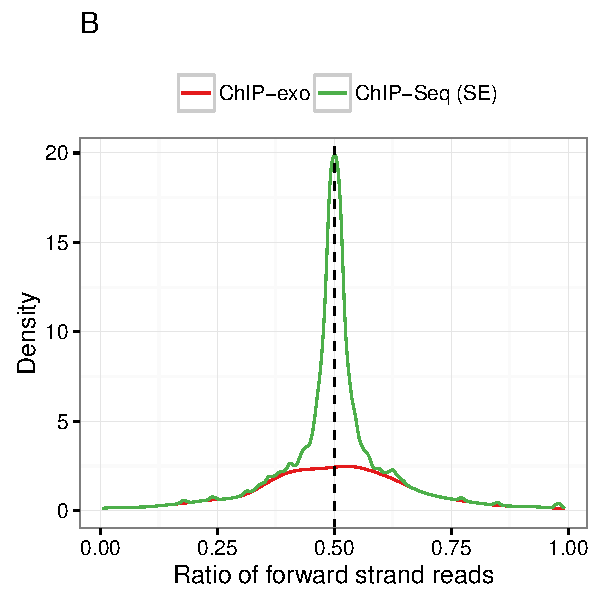
\includegraphics[width = .46\textwidth]{../figs/for_paper/forward_strand_ratio_comp_old.pdf}
  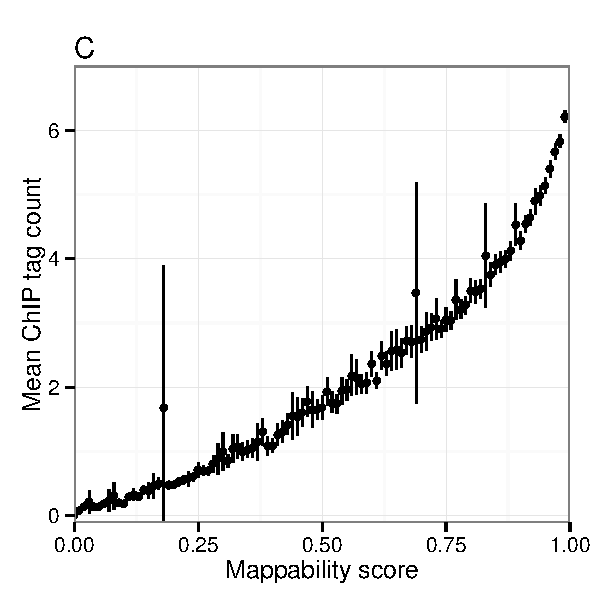
\includegraphics[width = .46\textwidth,page = 1]{../figs/for_paper/eukaryotic_bias_CTCF.pdf}
  \includegraphics[width = .46\textwidth,page = 2]{../figs/for_paper/eukaryotic_bias_CTCF.pdf}
  \caption{ A) ChIP signal in ChIP-exo was linearly related to that in
    PET ChIP-Seq data in the region with high ChIP tag counts. In
    contrast, there were clear differences in their background
    distribution, where several ChIP-exo background regions were
    empty. B) In ChIP-exo data, strands of reads were significantly
    less balanced in the regions with potential binding sites compared
    to SET ChIP-Seq data. C) ChIP tag counts increase linearly as
    mappability scores increases. D) ChIP tag counts increase linearly
    as GC content score increases when GC content is less than 0.6 and
    then ChIP tag counts decrease as GC content increases. }
  \label{fig:comp}
\end{figure}



We first compared various factors that could affect binding site
identification between ChIP-exo and ChIP-Seq data. In order to compare
distribution of signal and background between ChIP-exo and ChIP-Seq
data, we calculated ChIP tag counts across the genome by counting the
number of reads mapping to each of 150 non-overlapping
window after extending reads by 150 to their 3' end
directions. ChIP tag counts in ChIP-exo data were linearly related to
ChIP tag counts in ChIP-Seq data for the regions with high ChIP tag
counts (Figure \ref{fig:comp}A). This implies that signals for
potential binding sites are well reproducible between ChIP-exo and
ChIP-Seq data. On the other hand, there was clear difference in the
background distribution between them. In ChIP-Seq data reads were
almost uniformly distributed over background (non-binding) regions and
the ChIP tag counts in there regions were significantly larger than
zero. In contrast, in ChIP-exo data, there was larger variation in
ChIP tag counts among background regions and ChIP tag counts were much
lower in these regions compared to ChIP-Seq data. There were also
large proportion of regions without any read in ChIP-exo data. These
results indicate that background distribution of ChIP-exo data is less
homogeneous than that of ChIP-Seq data.

We next evaluated the ``peak pair'' assumption from Rhee and Pugh,
2011 \cite{exo1}, i.e. a peak of reads in the forward strand is
usually paired with a peak of reads in the reverse strand that is
located in the other site of the binding site. Wang et al., 2014
\cite{mace}, Madrigal 2015 \cite{cexor} and Bardet et al., 2013
\cite{peakzilla} proposed method rely in this assumption. In order to
evaluate this assumption, we reviewed the proportion of reads in the
forward strand in candidate regions (i.e. regions with at least one
binding site) in $\sig$ ChIP-exo data. We found that strands of reads
were much less balanced in ChIP-exo data than in ChIP-Seq data in
these regions with potential binding sites (Fig. \ref{fig:comp}B) and
this indicates that the peak pair assumption might not hold in real
ChIP-exo data.

We evaluated ChIP-exo data for CTCF factor from human genome
\cite{exo1} to investigate issues specific to eukaryotic genomes for
binding sites identification. Figures \ref{fig:comp}C and
\ref{fig:comp}D display the bin-level average read counts against
mappability and GC content. Each data point is obtained by averaging
the read counts across bins with the same mappability of GC
content. These results indicate that binding site identification in
ChIP-exo sample might also benefit from the use of methods that take
into account of apparent sequence biases such as mappability and GC
content.

\section{Results}
\label{sec:results}


\subsubsection{Comparison with ChIP-Seq data using dPeak}
\label{sec:dpeak_analysis}




Figure \ref{fig:reso_all} shows different comparisons among ChIP-exo,
PET ChIP-Seq and SET ChIP-Seq. A RegulonDB annotation was considered
identified if the distance between it and dPeak binding site estimate
was at most of 20 bp. That way, the sensitivity is defined as
the proportion of RegulonDB annotations identified in a peak. In
figure \ref{fig:reso_all}A can be seen that the sensitivity of all
protocols increases as the average distance between binding sites
does. Despite that when the binding events in a peak are closer to
each other, both ChIP-exo and PET ChIP-Seq are comparable, as the
distance increases ChIP-exo identifies a higher proportion of the
RegulonDB annotations; additionally SET ChIP-Seq is significantly less
sensible than both ChIP-exo and PET ChIP-Seq. In figure
\ref{fig:reso_all}B the distance between a RegulonDB annotation to its
closest prediction is compared for ChIP-exo, PET and SET ChIP-Seq;
while the first two are comparable, both outperform SET ChIP-Seq.

In figures \ref{fig:reso_all}C and \ref{fig:reso_all}D, we observe the
behavior of dPeak's estimated parameters for single end data (both
ChIP-exo and ChIP-Seq). The $\delta$ parameter measures the distance
from the 5' end of the fragment to its respective binding event and
the $\sigma$ parameter indicates the fragments distribution
variability around their respective binding sites (more information in
\cite{dpeak}). For both parameters, it can be seen that the ChIP-exo
estimates are smaller than the SET ChIP-Seq estimates in average,
which agrees with the fact that the sample reads are allocated more
tightly around the binding events in ChIP-exo data. Hence we can
conclude that the peaks shape is quite different between ChIP-exo and
SET ChIP-Seq.


\begin{figure}[h!]
  \centering
  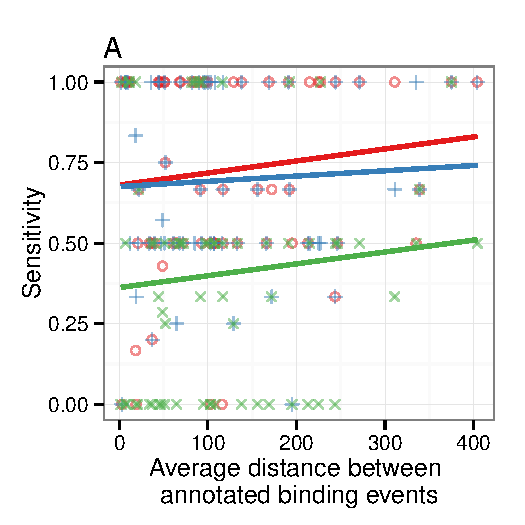
\includegraphics[width = .46\textwidth]{../figs/for_paper/sensitivity_exo_olda_data.pdf}
  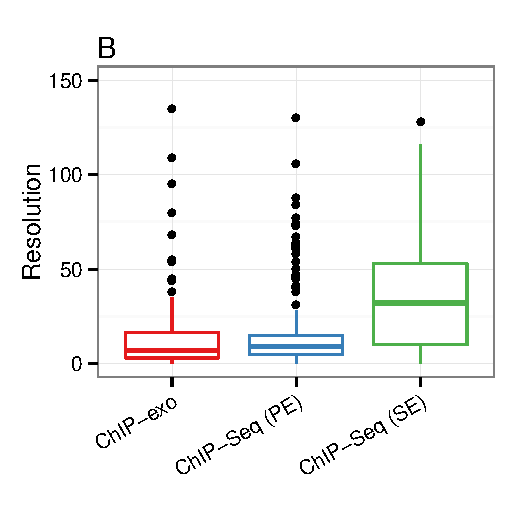
\includegraphics[width = .46\textwidth]{../figs/for_paper/resolution_by_dataset_old_data.pdf}
   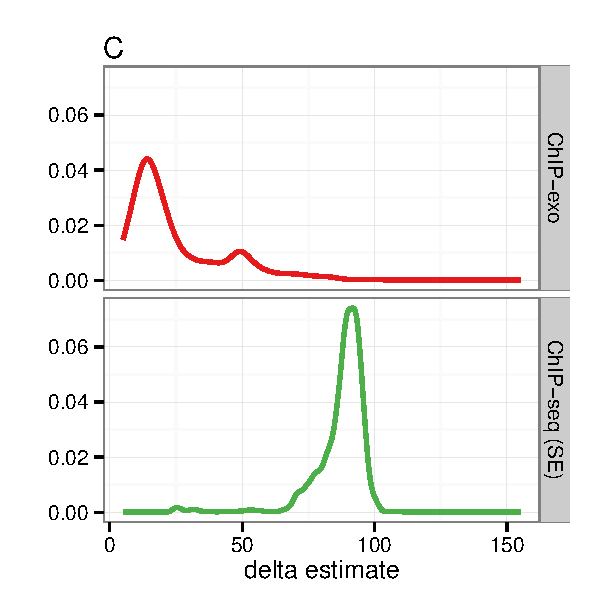
\includegraphics[width = .46\textwidth,page = 1]{../figs/for_paper/sigma_delta_old_densities.pdf}
   \includegraphics[width = .46\textwidth,page = 2]{../figs/for_paper/sigma_delta_old_densities.pdf} 

   \caption{Comparison of (A) sensitivity and (B) resolution between
     ChIP-exo and ChIP-Seq data. Sensitivity is defined as the
     proportion of RegulonDB annotations identified using each
     data. Resolution is defined as the distance between RegulonDB
     annotation and its closest prediction. $\quad$ C) $\delta$ parameter in
     dPeak measures average distance of the reads to their respective
     binding site. In ChIP-exo data, reads were located much closer to
     the binding site than in SET ChIP-Seq. D) $\sigma$ parameter
     measure the dispersion of reads around each binding site. In
     ChIP-exo data, reads showed less variation around the their
     respective binding sites compared to SET ChIP-Seq.}
  \label{fig:reso_all}
\end{figure}

\subsection{Recommendations for the design of ChIP-exo experiments}
\label{sec:reco}



We sampled a fixed amount of fragments for each of the ChIP-exo, PET
ChIP-Seq and SET ChIP-Seq datasets of the $\sigma^{70}$ sample in
aerobic conditions. For each sampled dataset we applied our
lower-to-higher resolution pipeline by calling peaks with MOSAiCS
\cite{mosaics} and then deconvolving the binding events by using dPeak
\cite{dpeak}. For the ChIP-exo datasets we called peaks by using
GC-content and mappability with MOSAiCS, and for the ChIP-Seq datasets
we used their respective Input samples.

\begin{figure}[h!]
  \centering
%  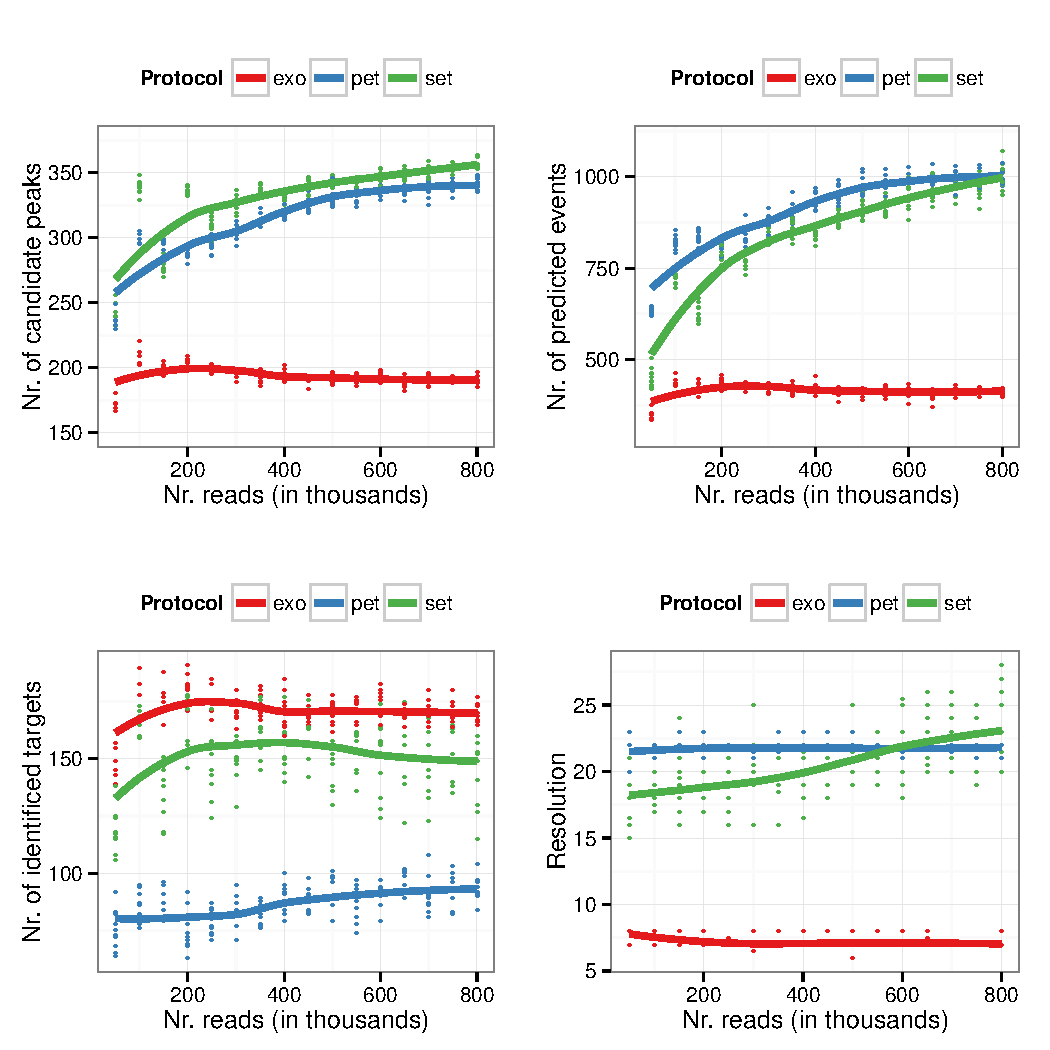
\includegraphics[width = .8\textwidth]{../figs/for_paper/Sig70_aerobic_saturation.pdf}
  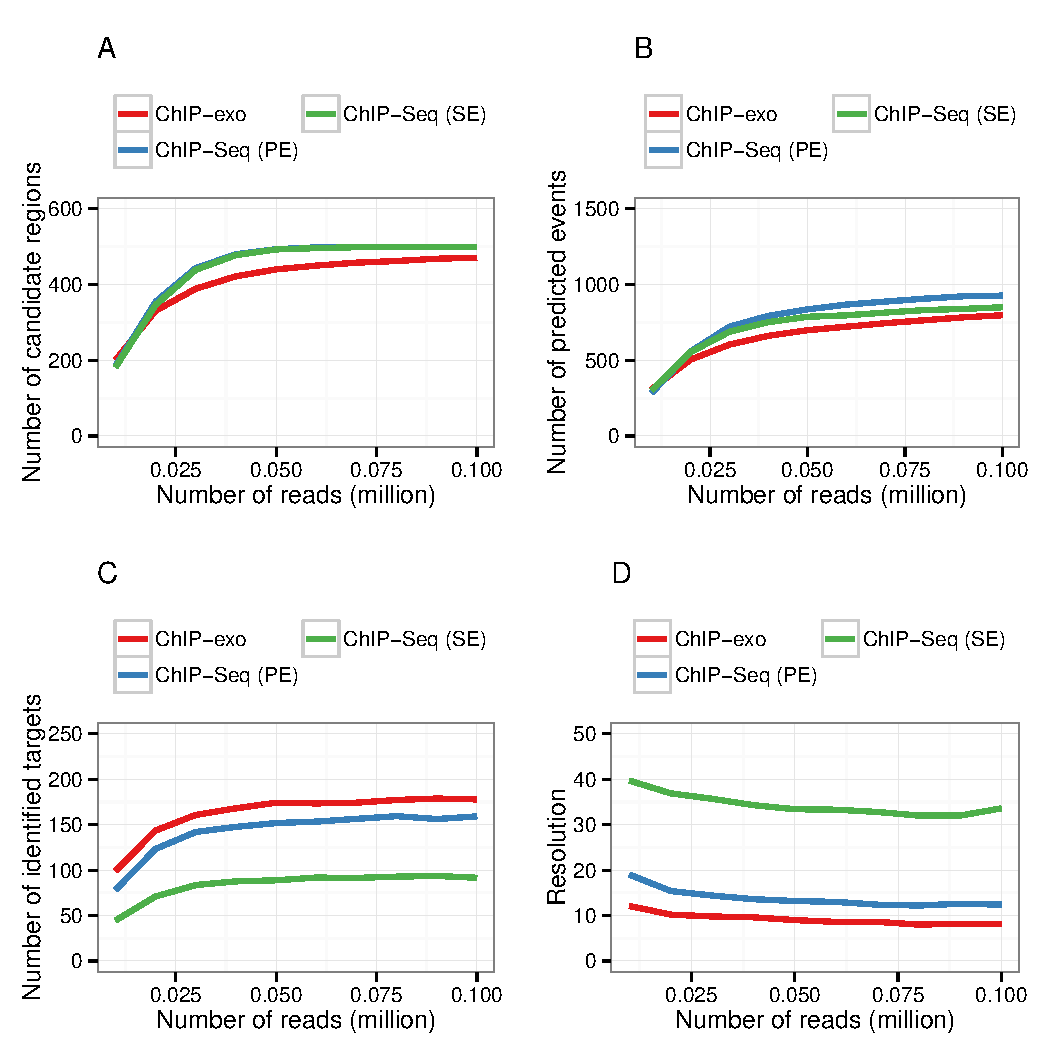
\includegraphics[width = .8\textwidth]{../figs/for_paper/saturation_analysis_old.pdf}
  \caption{Comparison of the number of candidate regions (A),
    predicted events (B), identified targets (C) and resolution (D)
    among ChIP-exo, PET ChIP-Seq and SET ChIP-Seq. RegulonDB
    annotations are considered as a gold standard. A gold standard was
    considered identified if a BS was estimated inside a 15
    bp window around it}
  \label{fig:design}
\end{figure}

Figure \ref{fig:design} shows the behavior of each data type when
their depth is fixed. It is remarkable that even when the number of
candidate peaks or the number of predicted events is lower for
ChIP-exo, it outperforms both PET and SET ChIP-Seq in the number of
identified targets and resolution. This may suggest that with ChIP-exo
less false positive peaks are being called and that when the targets
are being identified, dPeak estimates binding locations closer to the
true location. Additionally, we can see that as the read depth
increases all four indicators do so as well, which may indicate that
with ChIP-exo a smaller amount of reads is necessary to identify a
higher number of targets, but it may also be possible that this is an
artifact occurring due to ChIP-exo's lower library complexity.


\section{Conclusions}
\label{sec:conclusions}

We provide a ChIP-exo QC pipeline capable of assess the balance between
enriched samples and low complexity regions. It is shown that the
``peak-pair'' assumption doesn't hold in practice and we provide two
out-of-the-box visualization capable to assess the strand imbalance in
a ChIP-exo experiment.

We updated the dPeak algorithm from \cite{dpeak} and showed that
ChIP-exo is comparable in resolution and sensitivity with PET ChIP-Seq
and outperforms SET ChIP-Seq. ChIP-exo compared with PET and SET
ChIP-Seq at fixed depth sample is able to identify more targets at a
lower resolution. We compared dPeak with another algorithms to
estimate binding locations in ChIPexo data, dPeak is comparable to
MACE and outperforms GEM in resolution. dPeak provided a striking
balance in sensitivity, specificity and spatial resolution for
ChIP-exo analysis.


\newpage


\section{Planned work}
\label{sec:future}





\newpage

\bibliographystyle{plain} % Style BST file (bmc-mathphys, vancouver, spbasic).
\bibliography{chip_exo_paper}
\nocite{exo_gb}
\nocite{maplot1}
\nocite{maplot2}


\end{document}
